\chapter{Análisis de acumuladas}

El objetivo sigue siendo determinar cómo influye un idioma en otro,  y el analizar los préstamos nuevos no brindó información de las palabras que para 1900 ya formaban parte de los idiomas y que provenían de algún otro, es por ello que se ha decidido emplear a los préstamos acumulados.  

La simbología para las gráficas es la misma de la sección anterior, manteniendo las abreviaciones, los colores y el significado de las leyendas.  Nuevamente en el eje horizontal se localizan los años  entre 1900 y 2008, y en el eje vertical la frecuencia de uso; la gráfica resultante se nombrará como gráfica de uso del idioma A en el idioma B. 

Para ciertas combinaciones de idioma origen e idioma receptor, se han localizado más de cien palabras que conforman los préstamos del origen que se han acumulado en el receptor, ya que la búsqueda se realiza en cada año, el proceso de analizar palabra por palabra (como en los préstamos nuevos) y tratar de ligar a un evento histórico es inviable. La forma en que se presentarán los resultados es la misma que en el análisis de préstamos nuevos,  mostrando las gráficas de uso de A sobre B y la B sobre A; el hacer esto permitirá ver si hay cambios en las tendencias de las gráficas y si se presentan cruces de ellas.

\newpage
\section{Palabras acumuladas entre dos idiomas}

\subsection{Inglés y Francés}

\begin{figure}[h!]
	\centering
	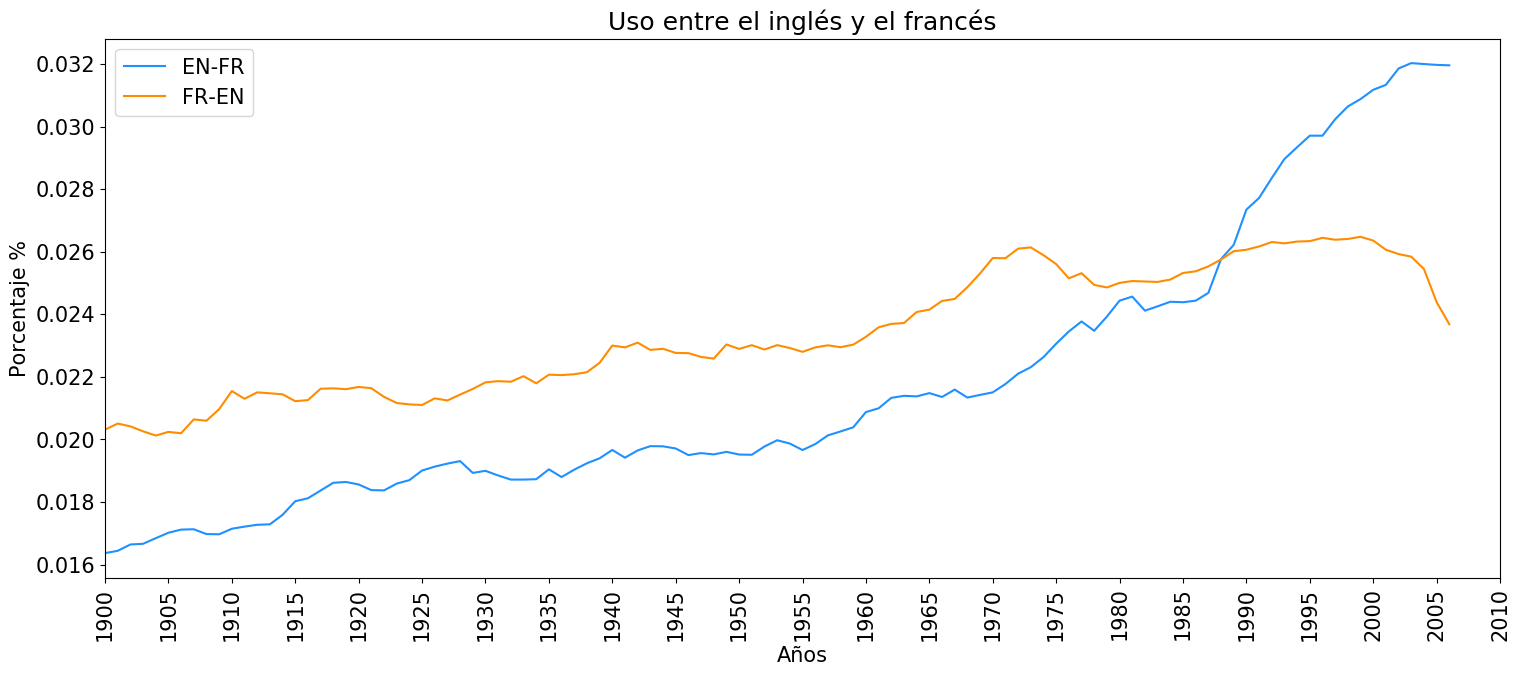
\includegraphics[scale=.38]{Cap_3/SF_1_S2_EN.png}
	\label{SF_EF}
	\caption{}
\end{figure}

Las gráficas de uso en ambos sentidos de los préstamos muestran una tendencia creciente desde el comienzo de las mediciones,  dominando el uso del francés en el inglés hasta 1990 donde se da el cruce de las gráficas para posteriormente ser los préstamos del inglés en el francés más utilizados que los de su contraparte.  A partir del cruce, es decir en los últimos veinticinco años, el inglés toma el lugar como idioma predominante despegándose en cada año que transcurre. 

Dentro de las palabras del inglés al francés que se han encontrado a partir del cruce en 1990 se encuentran internet, dollar, computer, communications, message, production;  palabras del campo semántico de la economía y la tecnología, disciplinas que se han favorecido una de la otra en los últimos años, y que han impulsado al inglés como un idioma común para la comunicación entre personas.  Otras palabras relevantes son Oxford y Cambridge,  ya que la extracción de palabras se obtuvo de los libros,  estas palabras muestran a ambas instituciones como líderes de editoriales, al ser los únicos nombres de editoriales en las listas.                         

El uso de los préstamos del francés en el inglés comenzó  a decaer tras el cruce siendo más evidente a partir del año 2000. Al analizar la lista de los préstamos, no hay cambios en las palabras que son más comunes por lo que a pesar de tener una palabra el mismo rango en las listas posteriores a la del año 2000,  su frecuencia disminuyó conforme transcurrieron los años; de forma generalizada el francés perdió importancia en el inglés en la primera década del siglo XXI.


\newpage
\subsection{Inglés y Alemán}

\begin{figure}[h!]
	\centering
	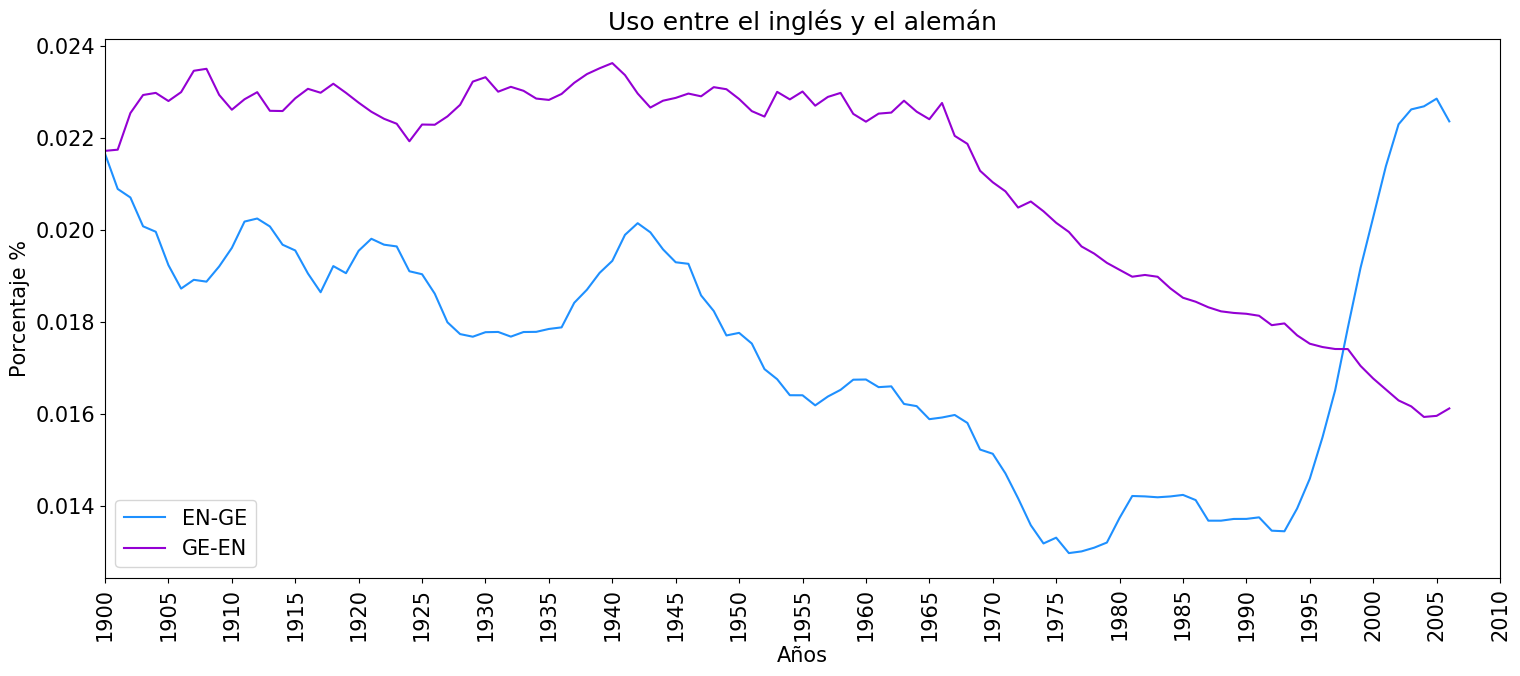
\includegraphics[scale=.38]{Cap_3/SF_2_S2_EN.png}
	\label{SF_EG}
	\caption{}
\end{figure}

En 1900 ambos idiomas eran igual de utilizados en el otro, pero al transcurrir el tiempo, las palabras del inglés comenzaron a ser menos utilizadas en los textos de alemán hasta alcanzar un mínimo de uso en 1990.  Al igual que en el francés, el aumento del inglés en el alemán comenzó a crecer después de 1990,  históricamente un año después de la caída del muro de Berlín, uno de los sucesos finales de los conflictos bélicos del siglo XX donde estuvieron involucrados países hablantes de ambas lenguas. La lista de préstamos acumulados muestra que las palabras ligadas a tales conflictos y que se catalogaron dentro de los préstamos nuevos de la sección anterior, están presentes en los años donde aumenta el uso del inglés en el alemán y continúan hasta el último año del análisis. Parte del gran crecimiento (de 0.014$\%$ a 0.024 $\%$) del inglés se asocia a la historia que compartieron ambos idiomas,  además los términos que involucran a la globalización como internet, mail, online, windows, marketing, financial, donde nuevamente los países hablantes de inglés o alemán han sido referentes en el desarrollo  científico y tecnológico de la primera década del dos mil.

El uso  del alemán en el inglés  se mantuvo en un umbral alrededor del 0.023 $\%$  por un periodo de casi sesenta y cinco años tras el cual comenzó su declive. Uno de los motivos de la pérdida del descenso en el uso es la situación que vivieron los países germanófonos en los años posteriores al término de la segunda guerra mundial,  donde la ideología política, la economía, los cambios territoriales y la intervención extranjera altera al idioma haciéndolo susceptible y debilitando su influencia ante los demás.  Este razonamiento puede ser arriesgado, sin embargo se planteará un algoritmo para decir en cual momento los idiomas son más propensos a perder  o ganar influencia en los demás.


\newpage
\subsection{Inglés e Italiano}

\begin{figure}[h!]
	\centering
	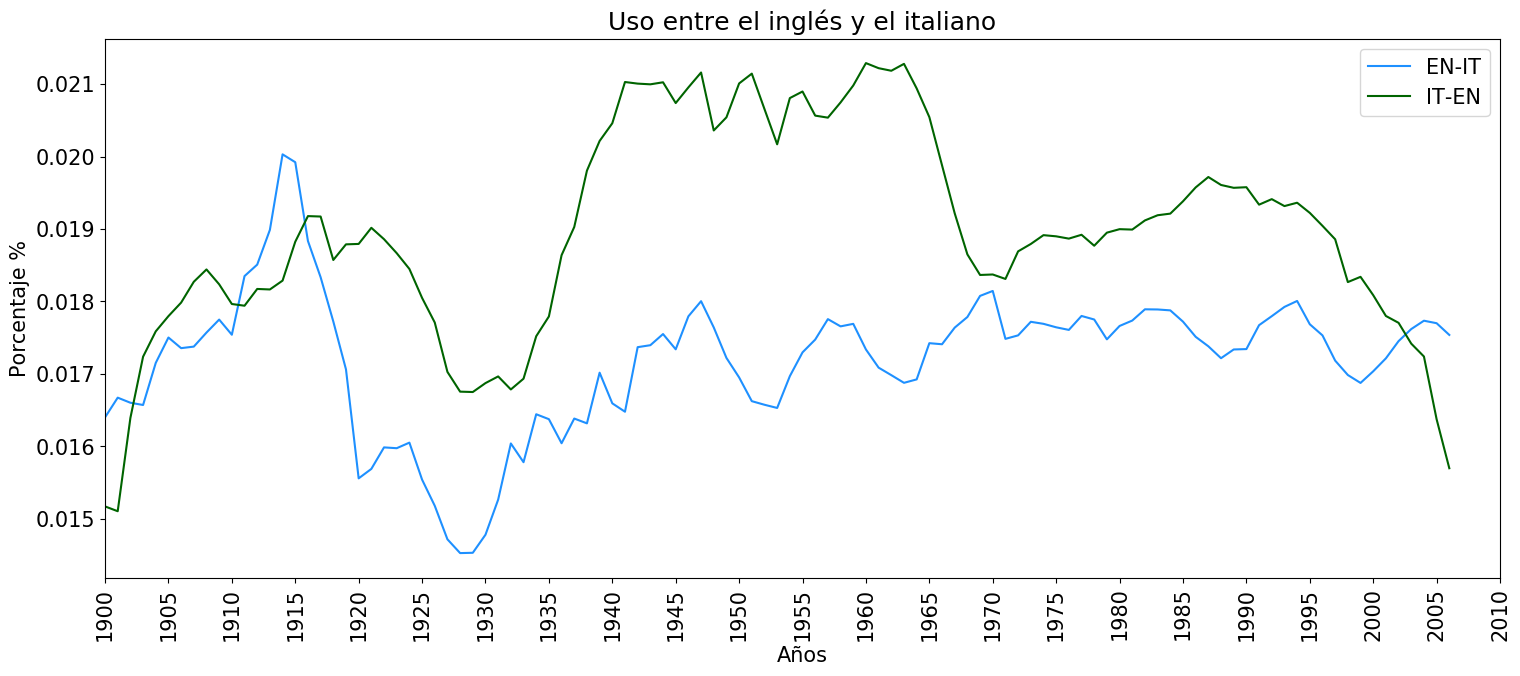
\includegraphics[scale=.38]{Cap_3/SF_3_S2_EN.png}
	\label{SF_EI}
	\caption{}
\end{figure}

Al retomar los resultados entre estos idiomas para los préstamos nuevos, las palabras del italiano al inglés no se lograron conectar a un hecho histórico que involucre a los dos idiomas, en los préstamos acumulados, el uso del italiano en el inglés predomina en un periodo más largo de tiempo (entre 1915 y el 2000) donde las palabras que constantemente aparecen son términos que provienen del griego y latín como test, inter, pure, format, regime, entre otras;  por lo que la influencia que tiene el italiano en el inglés se deben más a las raíces del italiano que también tiene el inglés.  

En el uso del inglés en el italiano,  hay dos periodos donde fue superior, el primero entre 1910 y 1915, donde el contenido predominante y que más se repite son verbos como be o do ( y sus diferentes conjugaciones),  el segundo periodo se da entre el 2000 y el 2005, donde la influencia del inglés supera a la del italiano, al igual que en los casos anteriores donde estuvo involucrado el inglés, predominan las palabras de los temas que abarcan a la globalización. 


\newpage
\subsection{Inglés y Español}

\begin{figure}[h!]
	\centering
	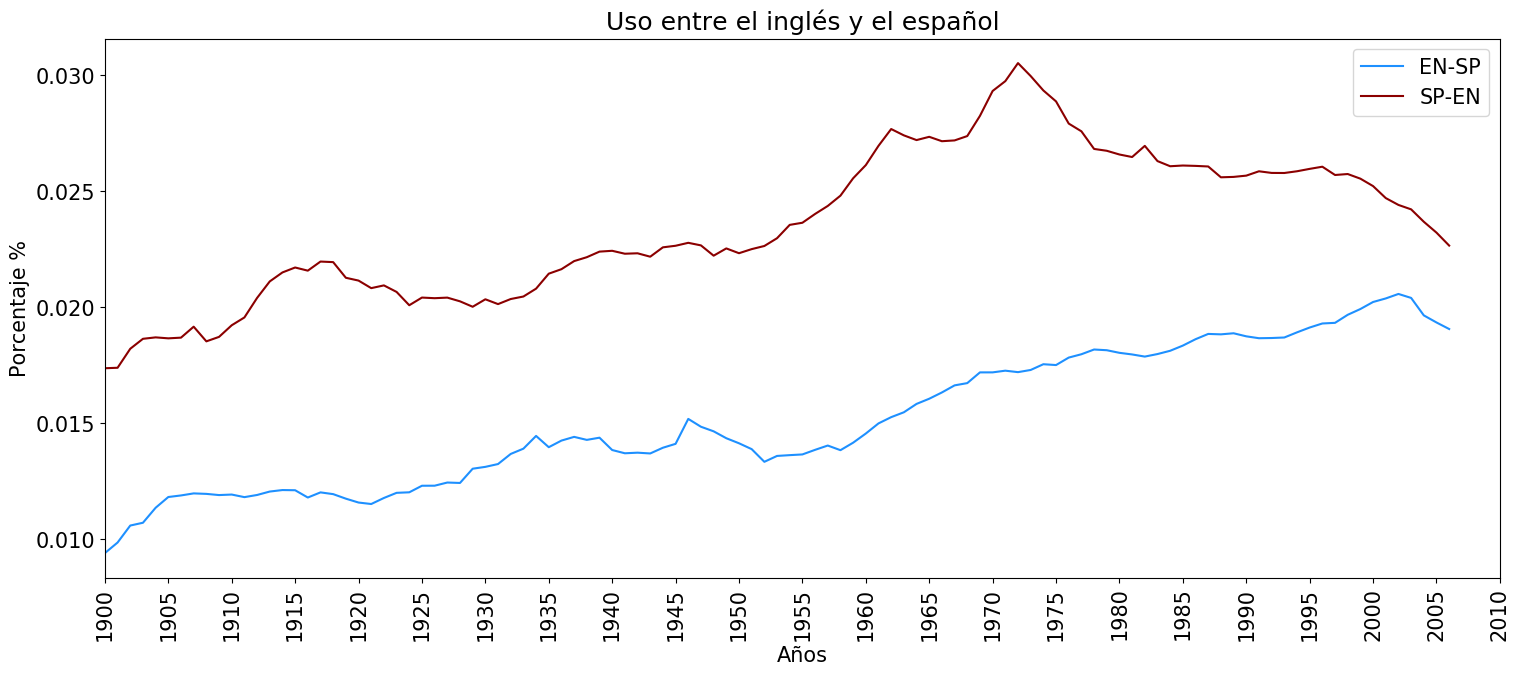
\includegraphics[scale=.38]{Cap_3/SF_4_S2_EN.png}
	\label{SF_ES}
	\caption{}
\end{figure}

El uso del inglés en el español es en todo momento menor,a diferencia de los resultados anteriores donde en algún periodo domina el uso del inglés.  En los más de cien años que se empleó el método el inglés creció desde un 0.01$\%$ hasta un casi 0.02$\%$, es decir casi 0.001$\%$ por cada década, siendo al momento el único caso donde el crecimiento es (casi) constante y no presenta un comportamiento repentino como el inglés en el francés o en el alemán a partir de 1990. No es viable decir que el crecimiento década a década continuará ocurriendo, ya que como se ha visto la espontaneidad de un evento modifica la forma en la que los idiomas interactúan entre sí, y el predecir la fecha de un suceso y el cómo afectará a los idiomas es imposible.  

Parte de las palabras que dan el incremento del uso del inglés en el español, se encuentran los verbos comunes del inglés be, do, have, estados y ciudades de Estados Unidos  como California, Texas, York, Chicago, y los términos relacionados al desarrollo global de los últimos años internet, mail, company.  Son importantes los nombres de ciudades y estados que aparecen, particularmente California y Texas, dos estados que concentran gran parte del producto interno de los Estados Unidos y la sede de industrias que más han crecido en los últimos años como la tecnológica,  la de energías, la aeroespacial y  la del entretenimiento; también son importante estos estados por la su historia con ambos idiomas, desde que el territorio de ambos pertenecía  a México,  su posterior anexión a los Estados Unidos por las guerras  de intervención,  y actualmente por ser lugares donde al radican inmigrantes ocasionando que la porción de la población de origen hispano aumente cada año. .

A pesar de los factores mencionados como responsables del crecimiento del inglés en el español,  el uso del español en el inglés es mayor , una razón de ello la da [XXXX] donde explica la tendencia del español antiguo a nacionalizar los términos que eran ajenos a él y que tuvo repercusiones aún en el siglo XX; es decir, si los conceptos que llegaban a España adoptaron una nueva escritura acorde al castellano,  reduciendo los préstamos (iguales en escritura)  y su uso en el español, al adoptarlos como propios. Si el nacionalizar palabras al español afectó a los demás idiomas, entonces el uso de cualquier idioma en el español es menor al uso del español en ese idioma, lo cual se comprobará en los siguientes resultados.



\subsection{Francés y Alemán}

\begin{figure}[h!]
	\centering
	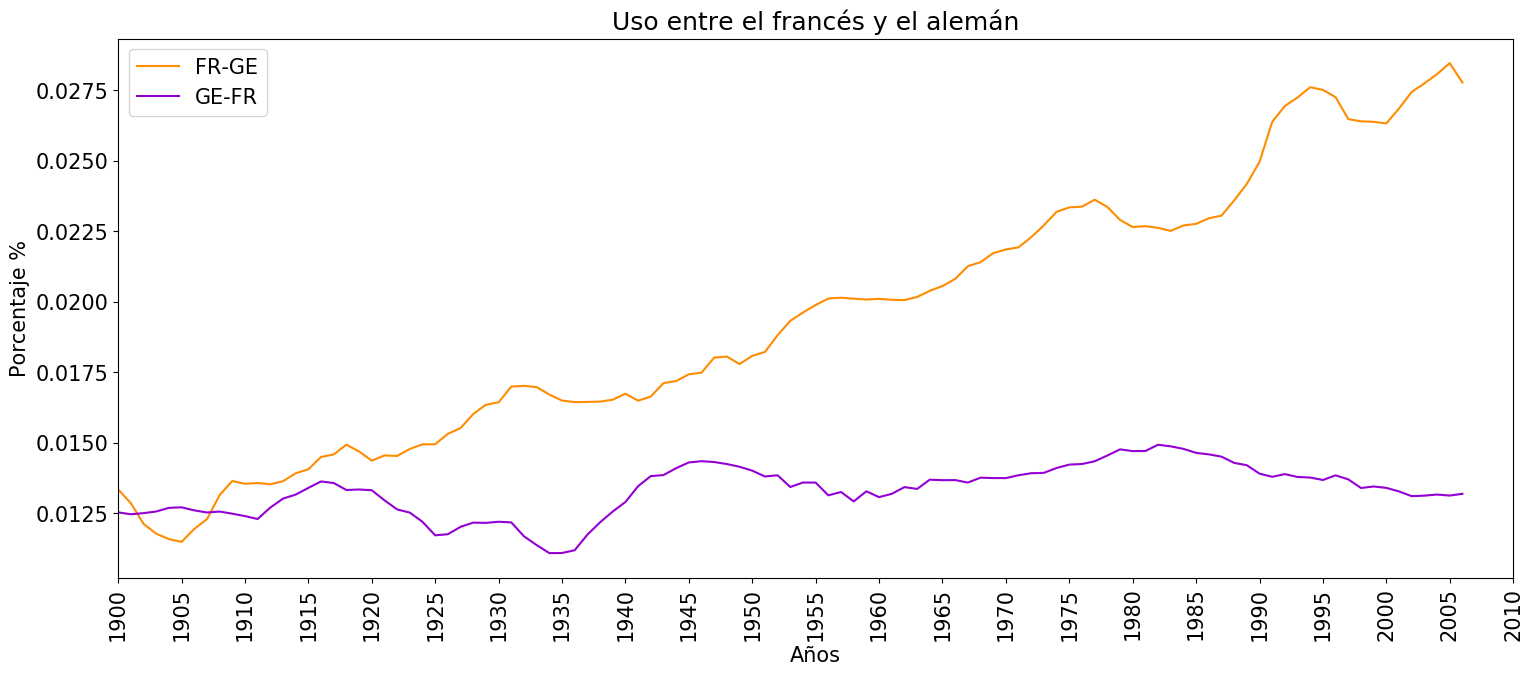
\includegraphics[scale=.38]{Cap_3/SF_2_S2_FR.png}
	\label{SF_FG}
	\caption{}
\end{figure}

Los préstamos provenientes del francés que recibe el alemán predominan en uso sobre los del alemán hacia el francés, aumentando la diferencia en cada año que transcurre.  En los años donde el alemán predominó sobre el francés (1900-1905) se encuentran términos médicos como anatomie, chirurgie, physiologie, psychologie y tuberculose, exponiendo cuán importante resultaron las investigaciones medicinas hechas en la Europa central.  En las listas posteriores comienzan a desaparecer los términos médicos, hasta que emerge la palabra Freud donde en cada año que aparece, también lo hace psychologie.  A pesar de que el crecimiento del alemán en el francés no es tan grande como en el sentido opuesto,  el año de 1935  hay otra erupción de palabras que repiten en cada año, estas ya se han mencionado en los préstamos nuevos y son referentes a la segunda guerra mundial. 

Los campos a los que se asocian los préstamos del francés al alemán son más diversos, desde la religión e ideologías políticas  en la primera mitad de siglo, hasta conceptos de la industria en la segunda mitad. Destaca que a pesar de los sucesos en los que se vieron involucrados países de habla francesa y alemana, el uso del francés ha sido creciente en el alemán  a pesar de la variedad de conceptos donde los préstamos son utilizados. 


\subsection{Francés e Italiano}

\begin{figure}[h!]
	\centering
	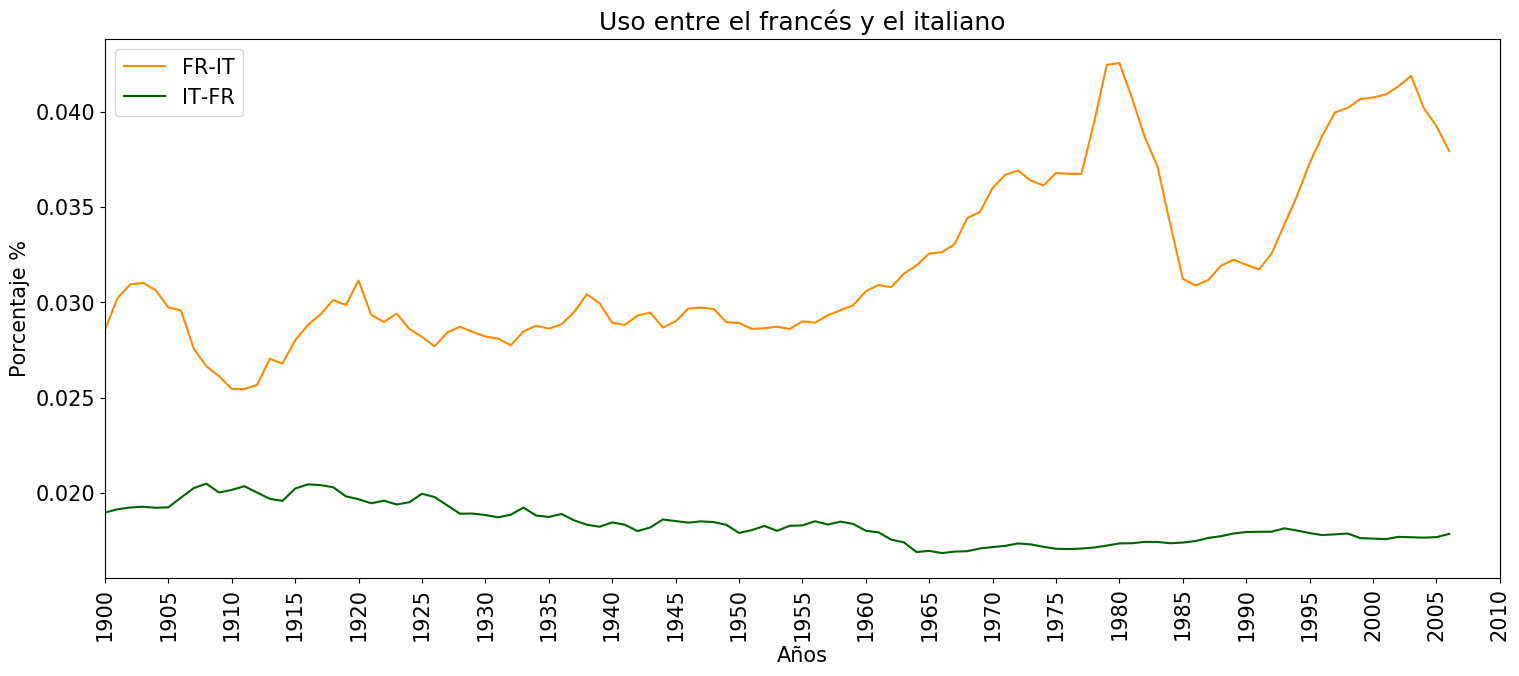
\includegraphics[scale=.38]{Cap_3/SF_3_S2_FR.png}
	\label{SF_FI}
	\caption{}
\end{figure}


El uso del francés en el italiano muestra tres periodos donde creció repentinamente, el primero entre 1915 y 1920, el segundo entre 1955 y 1980 y el tercero  entre 1990 y 2005.  La diversidad de tema donde pueden usarse los préstamos del francés en el italiano dificulta establecer una razón que explique los incrementos, el tener una variedad de temas caracterizó al francés como un idioma amplio  en contenido,  ya que la misma propiedad se encontró para los préstamos del francés al alemán.  Un factor general para los incrementos en el tercer periodo se debe a la globalización,  por la erupción de palabras  técnicas afines al área (economie, industrie,  capitale) aunque estas se encuentren en otros idiomas, son constantemente repetidas en las listas desde 1991 hasta 2007. 

Al analizar los préstamos en sentido opuesto, es decir los que van del italiano al francés,  la gráfica no presenta modificaciones drásticas en su uso,  siempre manteniéndose alrededor del 0.02$\%$. El contenido muestra vocablos que relacionan a los países de Italia y Francia, como lo es la palabra vigne  (traducción de viñedo) que vincula la industria vitivinícola donde ambos países tienen presencia

\newpage
\subsection{Francés y Español}


\begin{figure}[h!]
	\centering
	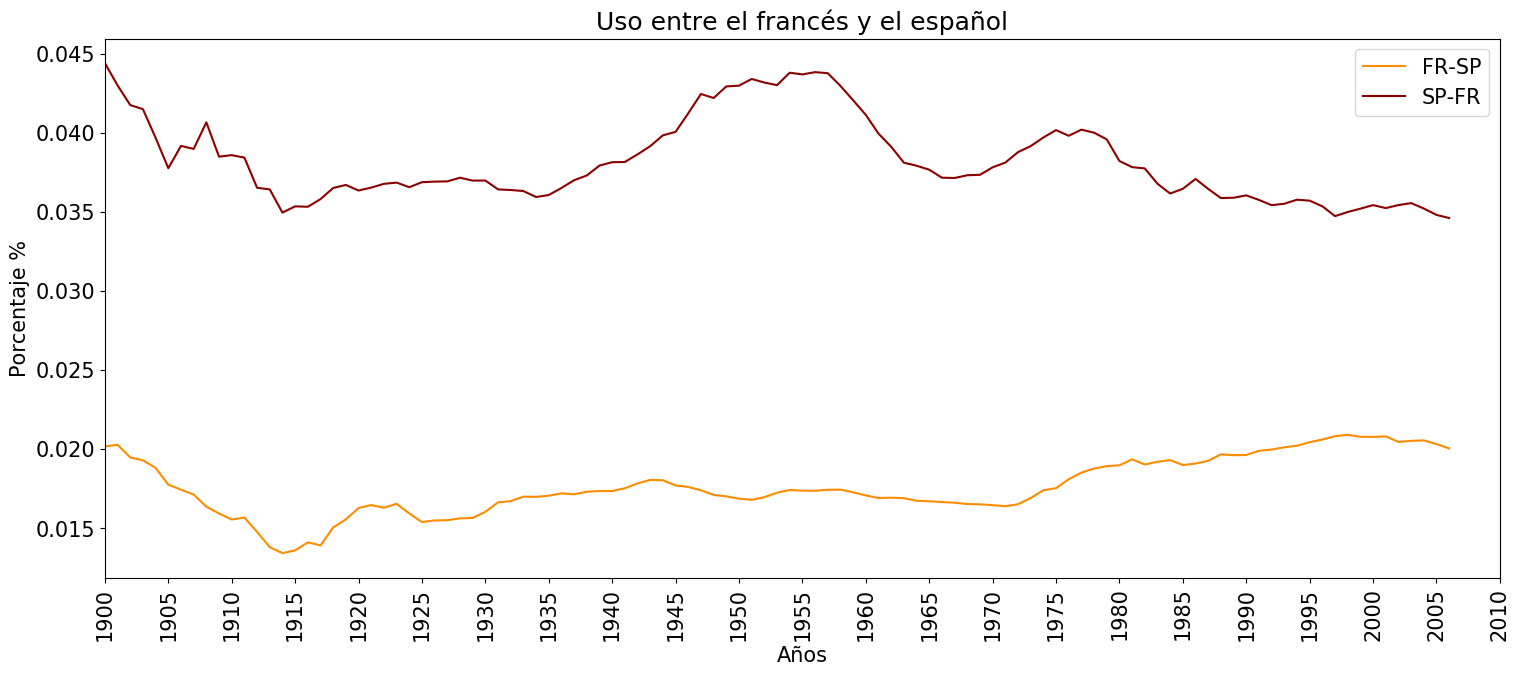
\includegraphics[scale=.38]{Cap_3/SF_4_S2_FR.png}
	\label{SF_FS}
	\caption{}
\end{figure}



Entre ambos idiomas, el español ha sido más utilizado en el francés durante el siglo pasado,  teniendo en cada década una diferencia del 0.02$\%$ , aunque hay una diferencia entre los usos, la lista de préstamos en ambos idiomas receptores muestran palabras que difícilmente podrían ser catalogadas como préstamos, es decir ya son palabras que por su familiaridad con el idioma receptor ya es común pensarlas como si siempre hubiesen formado parte del idioma.   

Una razón de la familiaridad entre el francés y el español se da por  provenir ambas de la familia de las lenguas romances, donde la mayoría de las palabras tienen el mismo origen etimológico dificultando el responder quien ha tenido una mayor influencia. Por la antigüedad de los mismos idiomas y su relación común en el greco latin, sí existió un periodo donde la adopción de nuevas palabras modificó el uso de los idiomas, tal período puede ser igualmente antiguo y las palabras nuevas se han adaptado al receptor de tal forma que siguen la tendencia del uso del mismo, es decir el uso de  la palabra “París” en el español se comporta como el uso de todas las palabras en español sin importar su distinción si provienen de un idioma determinado o son de origen español.  Esta premisa se verificará en las últimas secciones del escrito y se espera se cumpla para las lenguas romances del trabajo ( francés italiano y español)



\newpage
\subsection{Alemán e Italiano}

\begin{figure}[h!]
	\centering
	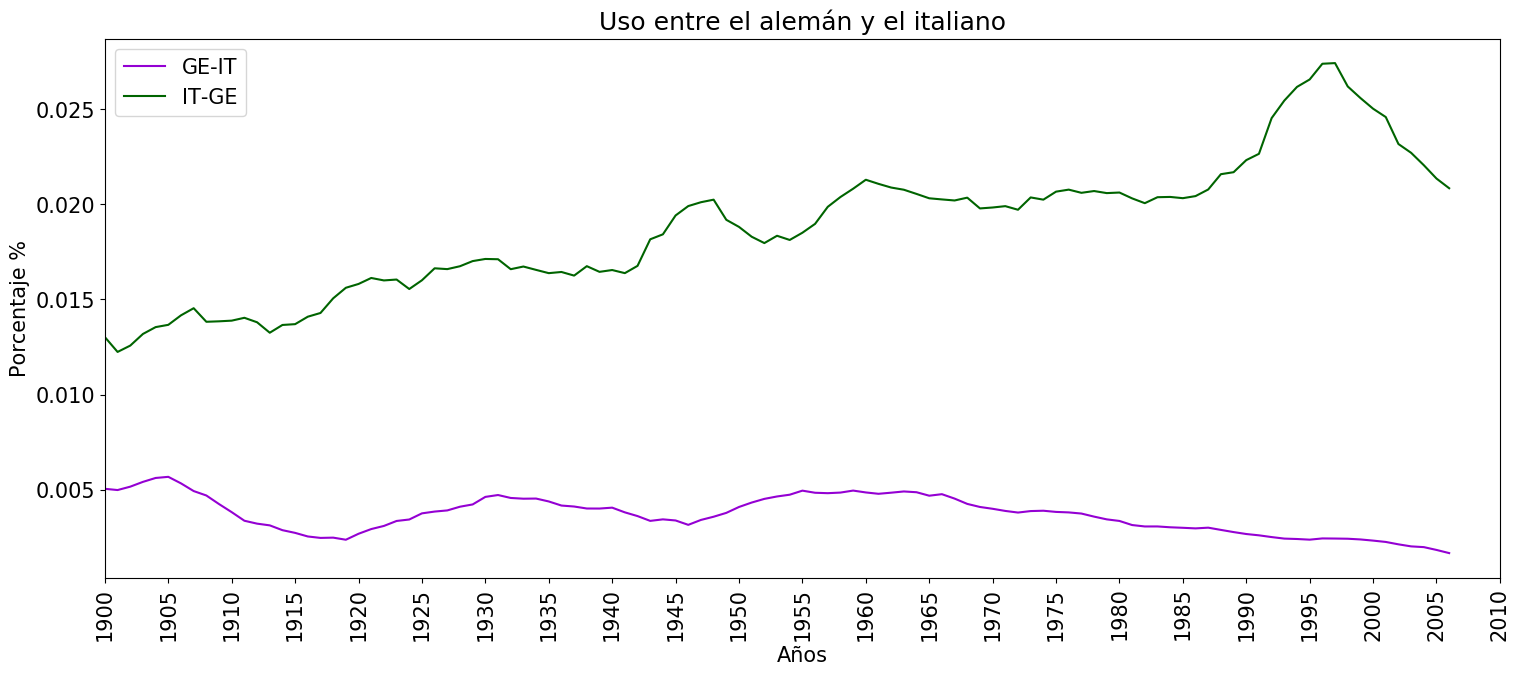
\includegraphics[scale=.38]{Cap_3/SF_3_S2_GE.png}
	\label{SF_GI}
	\caption{}
\end{figure}

El uso del italiano en el alemán ha incrementado en el siglo XIX, por la historia entre las naciones con estos idiomas oficiales,  destaca nuevamente la presencia de la palabra Mussolini  continuamente desde 1935 hasta 1953, y alternando periodos de aparición de uno o dos años  con desapariciones por el mismo tiempo. En los mismos años donde aparece Mussolini se encuentran las palabras de regime, status, schema, liberale y Ribbentrop  (estas palabras ya se habían tratado en los préstamos nuevos) en diferentes posiciones de rango pero dentro de la misma lista; el tener este conjunto del mismo campo semántico, que dentro de los años de aparición haya sucedido la segunda guerra mundial y que el uso del italiano en el alemán haya aumentado y disminuido en casi las mismas fechas hace posible las conexiones entre estas variables, es decir la guerra propició a que las palabras relacionadas al conflicto alterarán el uso del italiano en el alemán.    El último incremento se dio antes del año 2000,  siendo una característica que el alemán ha presentado en los análisis anteriores, el inglés  y francés también crecieron antes del año dos mil en el alemán, por lo que debe de ser una tendencia general del idioma alemán el crecer en esta fecha. 

Los préstamos del alemán no muestran un cambio relevante en la forma en que son utilizados en el italiano,  pero si hay diferencias entre el contenido de las listas en las dos mitades de siglo,  destacan en la primera mitad ciudades alemanas como Berlín, Leipzig, y en la segunda los apellidos de personajes germanófonos mencionados en los préstamos nuevos.  La presencia de los apellidos, muestra la relevancia que lograron los personajes en sus respectivos campos,  al ser constantes en las listas. 


\newpage
\subsection{Alemán y Español}

\begin{figure}[h!]
	\centering
	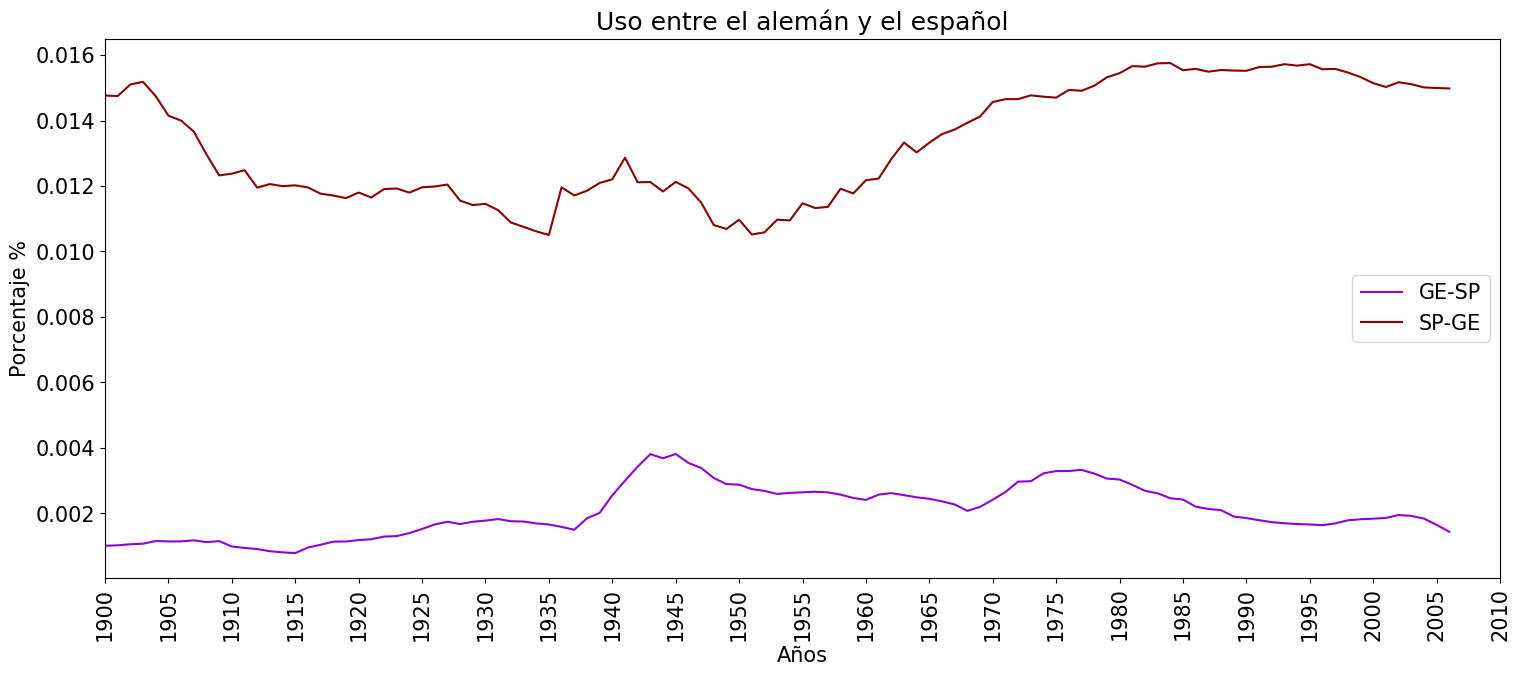
\includegraphics[scale=.38]{Cap_3/SF_4_S2_GE.png}
	\label{SF_GS}
	\caption{}
\end{figure}

Entre el uso de un idioma en el otro,  es escaso el utilizar palabras del alemán en el español, siendo el más pequeño  (entre el 0.002$\%$ y 0.004$\%$) entre todas las combinaciones hechas, su mayor ascenso comenzó en 1935 y su estabilidad se dio de 1945 a 1985,  épocas donde los pueblos germanófonos y sus hablantes  fueron citados por su papel en la historia y las consecuencias que originaron en diferentes ámbitos.  Dentro de las palabras que no se han mencionado, se encuentran metal y mineral,  donde estas fueron clasificadas como de origen alemán por ser el idioma donde tenían más relevancia al principio de las mediciones, aparecen en el español  por ser  la industria metalúrgica una de las actividades que caracterizaron a los países hispanos como productores, y su importancia en el alemán por ser la misma industria una de las bases de la revolución industrial alemana en el siglo XIX. 

El periodo donde los préstamos del español al alemán comenzaron a aumentar también comienza en 1935  manteniendo la misma tendencia hasta 1945,  coincidiendo con el pequeño apogeo del alemán en el español.  La lista de palabras no muestra coincidencias entre las palabras y el evento bélico de la época, sin embargo las palabras más repetidas a partir de ese año de crecimiento son  general, américa, capital, europa y washington, términos que bien pueden ser usados dentro del mismo contexto histórico de la postguerra. 



\newpage
\subsection{Italiano y Español}

\begin{figure}[h!]
	\centering
	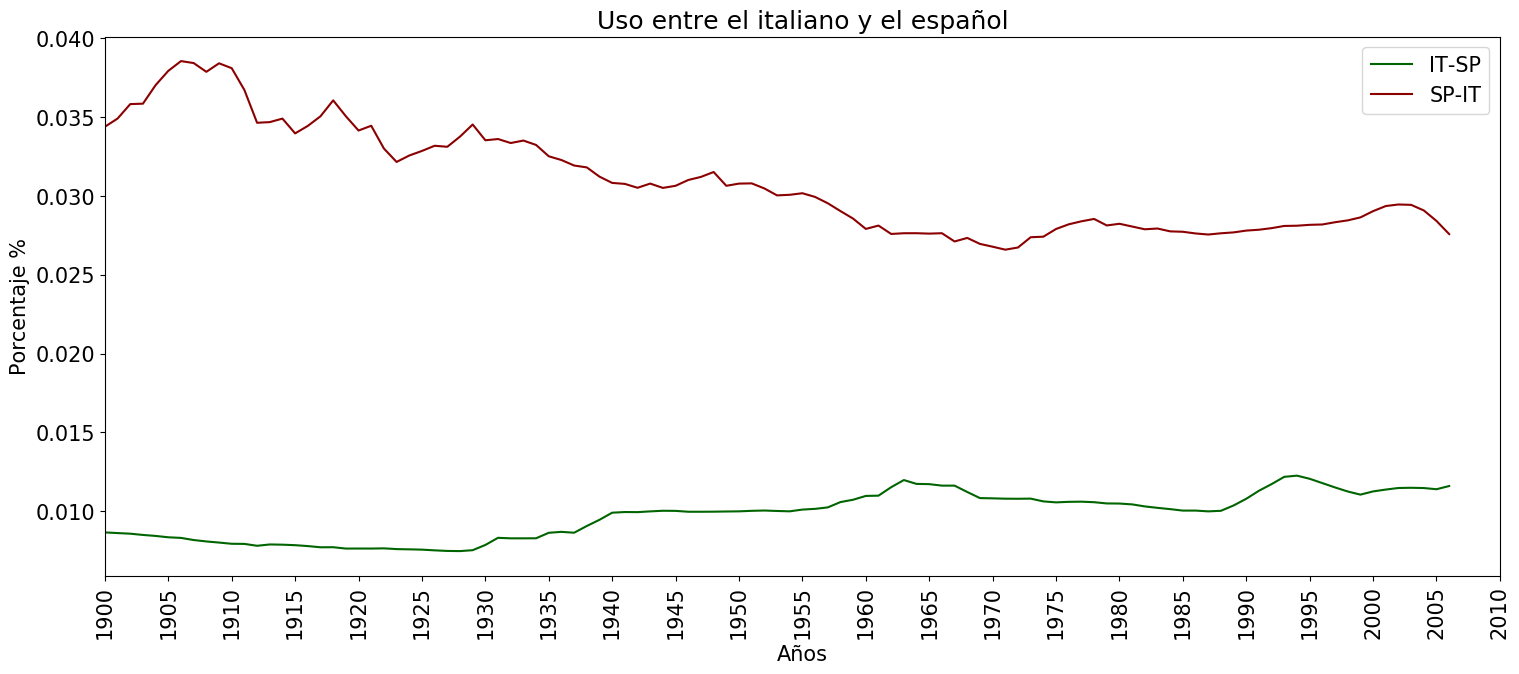
\includegraphics[scale=.38]{Cap_3/SF_4_S2_IT.png}
	\label{SF_IS}
	\caption{}
\end{figure}

El comportamiento entre estos idiomas es similar al calculado entre el francés y el español, donde el uso del español predomina.  Nuevamente se están tratando dos lenguas romances  que comparten muchas palabras de la misma rama etimológica y donde una palabra puede ser común en el receptor aunque se haya clasificado como nueva o de un determinado origen.     

De estas palabras catalogadas como de origen español,  a pesar de ser ampliamente utilizadas en el italiano, su uso ha decaído aunque esta puede ser una tendencia del italiano por sí mismo ya que el comportamiento de los demás idiomas en el italiano ha decaído en los últimos veinticinco años (desde 1985). 

Por parte de los préstamos del italiano usados en el español,  su uso aunque mínimo ha incrementado desde 1930,  parte de este incremento pueden ser por el auge en publicaciones de américa latina,  al encontrar palabras como realismo, latina, o narrativa, además de los  términos asociados a ideologías políticas que igualmente ya se comentaron en los préstamos nuevos del italiano al español, y que perduraron en el siglo pasado.



\newpage
\section{La cantidad de préstamos acumulados y el uso en conjunto}

En los comentarios pasados  se ha mencionado las palabras que forman parte de las listas de los préstamos acumulados, y como algunas de ellas han logrado modificar el uso de un idioma en otro. También se ha especificado que el uso de un idioma en otro se obtiene por la frecuencia de las palabras que conforman la lista, más no por la cantidad de ellas. Para aclarar esta hipótesis,  se realizó la tabla [XXXX]]] mostrando el promedio de palabras con origen A que se encuentran en las listas de B. 

\hfill\break

\begin{table}[h!]
	\centering
	\begin{tabular}{lcccccc}
		\multicolumn{7}{c}{R E C E P T O R}                                                                                                                                             \\
		\multirow{6}{*}{\begin{tabular}[c]{@{}l@{}}O\\ R\\ \,I\\ G\\ E\\ N\end{tabular}} &             & \textbf{EN} & \textbf{FR} & \textbf{GE} & \textbf{IT} & \textbf{SP} \\
		& \textbf{EN} & -           & 324.43      & 164.33      & 77.5        & 73.61       \\
		& \textbf{FR} & 297.36      & -           & 94.06       & 118.55      & 66.31       \\
		& \textbf{GE} & 63.87       & 48.06       & -           & 34.92       & 16.61       \\
		& \textbf{IT} & 77.82       & 100.62      & 47.9        & -           & 219.45      \\
		& \textbf{SP} & 118.43      & 84.22       & 29.85       & 311.97      & -          
	\end{tabular}
	\caption{}
	\label{T_PA}
\end{table}




De la tabla se aprecian dos relaciones similares entre la cantidad de palabras, la primera entre el inglés y el francés si se escoge uno de estos dos idiomas como el idioma origen, entonces el otro funge como el receptor donde las palabras del origen son mayoritarias; la misma característica ocurre con el italiano y el español.  Las relación entre el español y el italiano es esperada, al provenir ambas de la familia de las lenguas romances, la composición etimológica de sus vocablos es semejante,  resultando en una mejor adaptación en el idioma receptor. 

Ahora para decir con seguridad cuál idioma es más influyente en otro,  se realizarón dos gráficas de influencia en conjunto, para ello se requirió de un idioma origen A y de los diferentes idiomas receptors B, C, D y E.  La primera gráfica consiste en ver  el uso de los préstamos de A que llegan a los diferentes receptores pero visualizados todos en una misma gráfica,  es decir estará el uso de A en B, el de A en C y así sucesivamente,  con ello se determina y por cuáles periodos  A es más influyente.   La segunda gráfica de conjunto, se intercambian los idiomas receptores por orígenes, y se grafican el uso de los demás idiomas en el idioma receptor A, para  sostener el argumento de cual idioma ha influenciado más al idioma A.       

Lo interesante de estas gráficas es que  muestra todos los comportamientos de un idioma en los demás, y de los demás en el idioma,  ya no es solo ver los préstamos de A en B y los de B en A. La tabla anterior es útil para ver que en pocos casos se cumple que el idioma que más palabras tiene es el más utilizado. 

\newpage
\subsection{Inglés}


\begin{figure}[h!]
	
	\begin{subfigure}{}
		\centering
		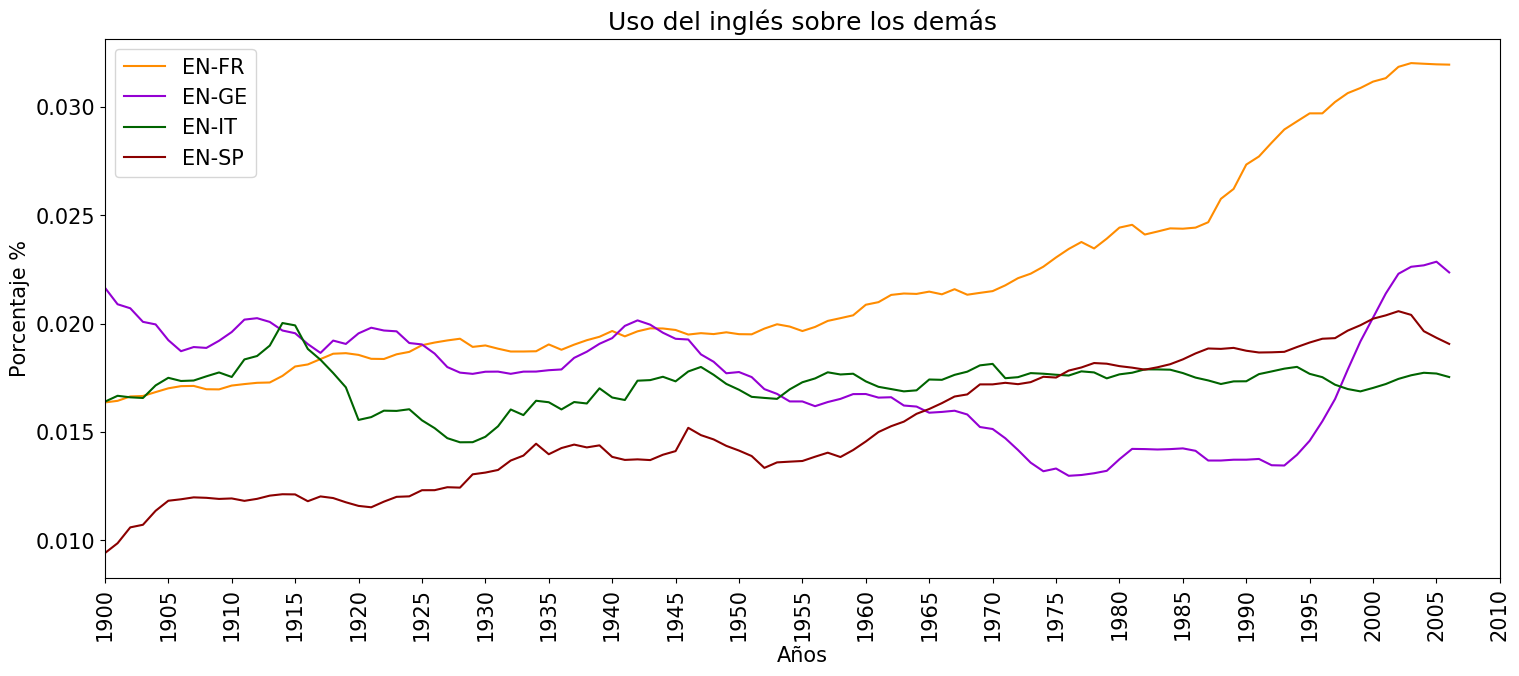
\includegraphics[scale=.38]{Cap_3/PF1_S2_EN.png}
		\caption{}
		\label{fig:ST_EN_a}
	\end{subfigure}
	
	\begin{subfigure}{}
		\centering
		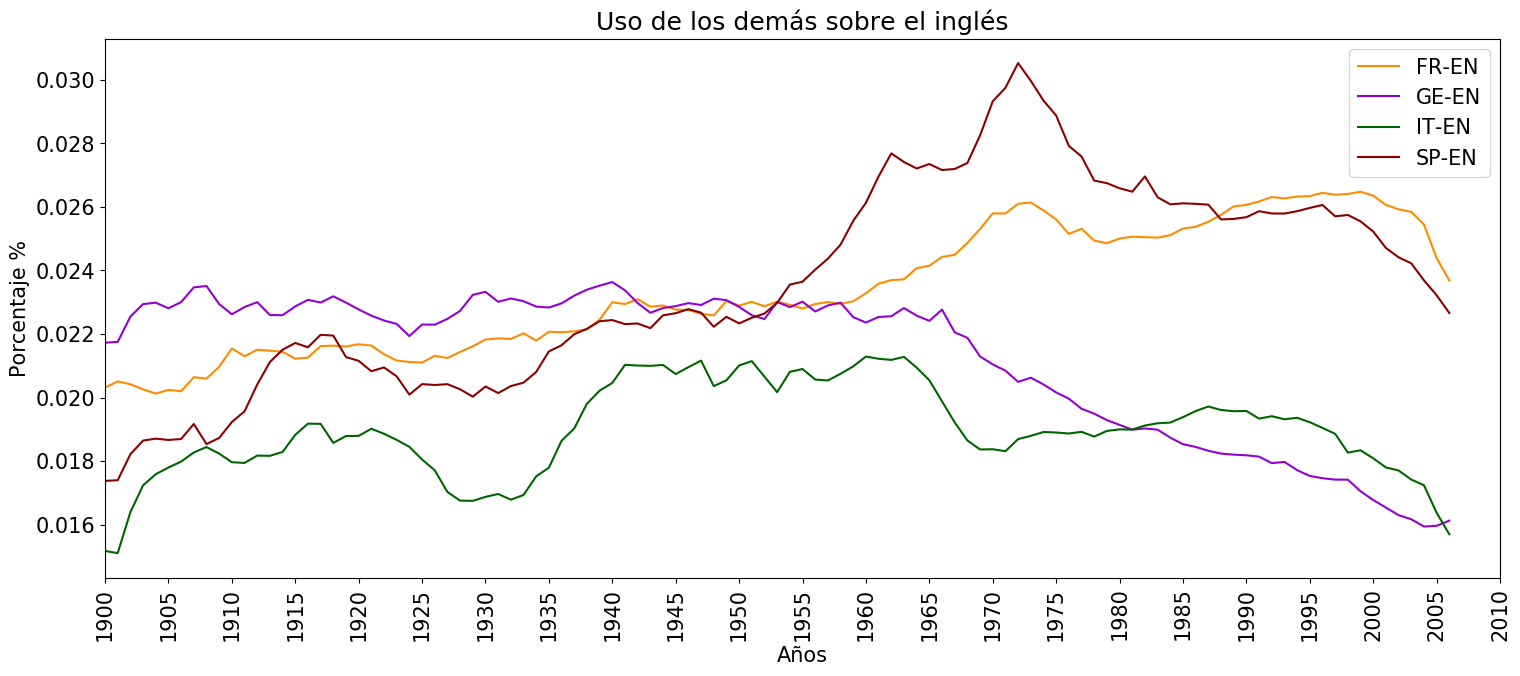
\includegraphics[scale=.38]{Cap_3/PF2_S2_EN.png}
		\caption{}
		\label{fig:ST_EN_b}
	\end{subfigure}
	
\end{figure}


Tomando al inglés como idioma origen, antes de 1945 su uso era similar entre el francés, el alemán y el italiano. Involucrando a la historia en la razón del crecimiento,  Alemania e Italia  fueron dos de los países perdedores de la segunda guerra mundial, por otra parte Estados Unidos (mayoritariamente), el Reino Unido y Francia se catalogaron como vencedores; siendo el periodo posguerra donde Estados Unidos se revalorizó como un país con poderío armamentista, con presencia en múltiples industrias, y con un modelo económico estable y que hasta el momento la mayoría de los países utiliza, incentivando el uso del inglés como idioma común entre países; el aspecto económico se refleja en en la gráfica del alemán, donde el incremento del inglés se da en años posteriores a 1990 donde en Alemania se termina el uso del otro modelo económico, con la disolución de la Unión Soviética, y donde comienza el dominio del mercado estadounidense con la cotidianidad de la tecnología y el internet. 

Aspectos como la proximidad geográfica entre Estados Unidos con Latinoamérica,  el aumento de las migraciones de personas entre ambos costados (siendo mayor el flujo hacia Estados Unidos),  las relaciones diplomáticas y de mercado surgen como posibilidades no solo del crecimiento del inglés en el español, sino también en el sentido opuesto, del español en el inglés, reflejado en el segundo gráfico, donde el español alcanza su punto más alto en 1970, de acuerdo a [XXXXXX] año donde se dio el mayor flujo de migrantes a Estados Unidos,  y a partir de donde empezó a crecer la comunidad hispana en el país. 


En el segundo gráfico,  el uso de los demás idiomas en el inglés se estabiliza entre los vales de  0.020$\%$ y 0.024$\%$  en los años de 1940 y 1955,  nuevamente, período que comprende el término de la segunda guerra mundial, el comienzo de la guerra fría y la división del mundo en dos bloques económicos,  salvo por el español que comenzó a ser el idioma más usado en el inglés a partir de 1950 (aspecto ya mencionado), mientras que los demás idiomas continúan con la misma relevancia  hasta principios de 1960.  De forma general el uso en el inglés decae en  1990 a partir de que el modelo económico de Estados Unidos es empleado por la mayoría de los países,  asimismo surge el desarrollo en las telecomunicaciones,  la globalización y nuevas herramientas como el internet, todas ellas donde el inglés es el medio natural para transmitir y compartir información. 


\newpage
\subsection{Francés}

\begin{figure}[h!]
	
	\begin{subfigure}{}
		\centering
		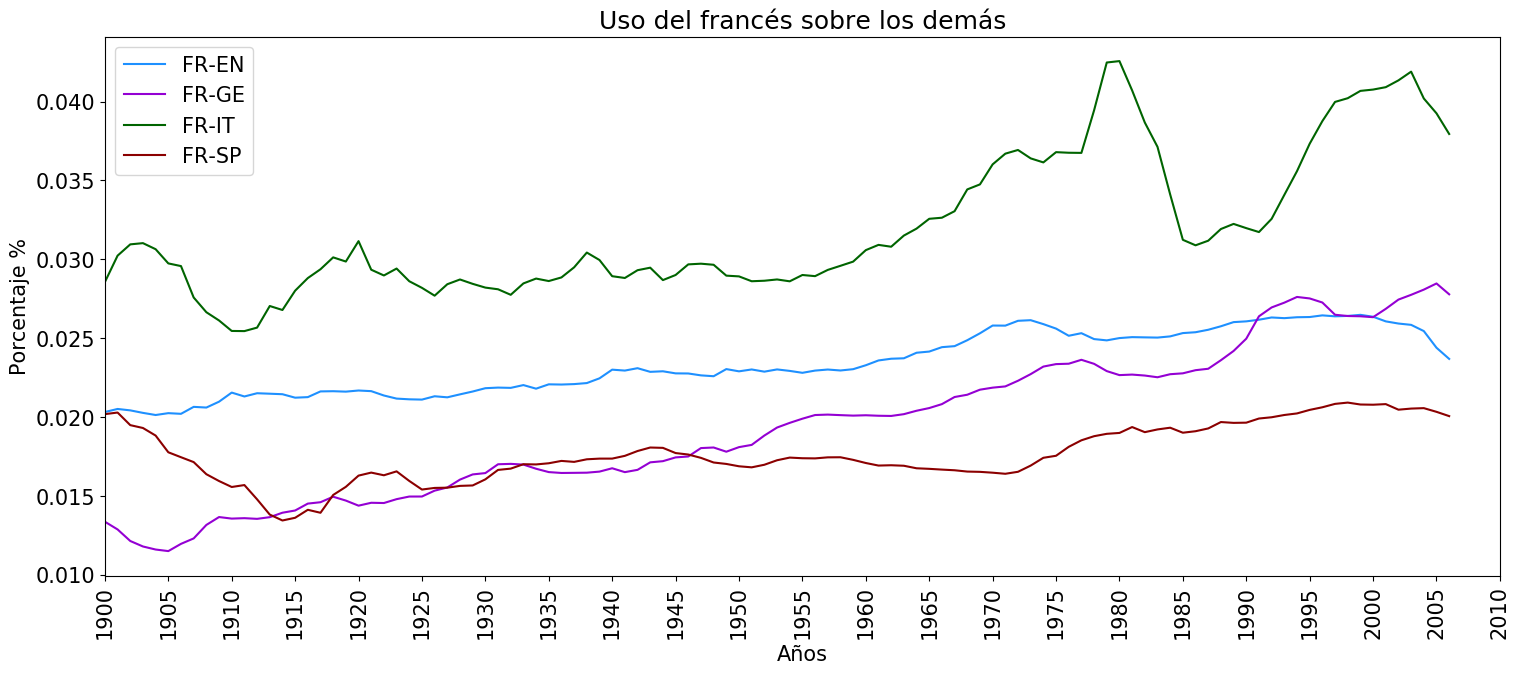
\includegraphics[scale=.38]{Cap_3/PF1_S2_FR.png}
		\caption{}
		\label{fig:ST_FR_a}
	\end{subfigure}
	
	\begin{subfigure}{}
		\centering
		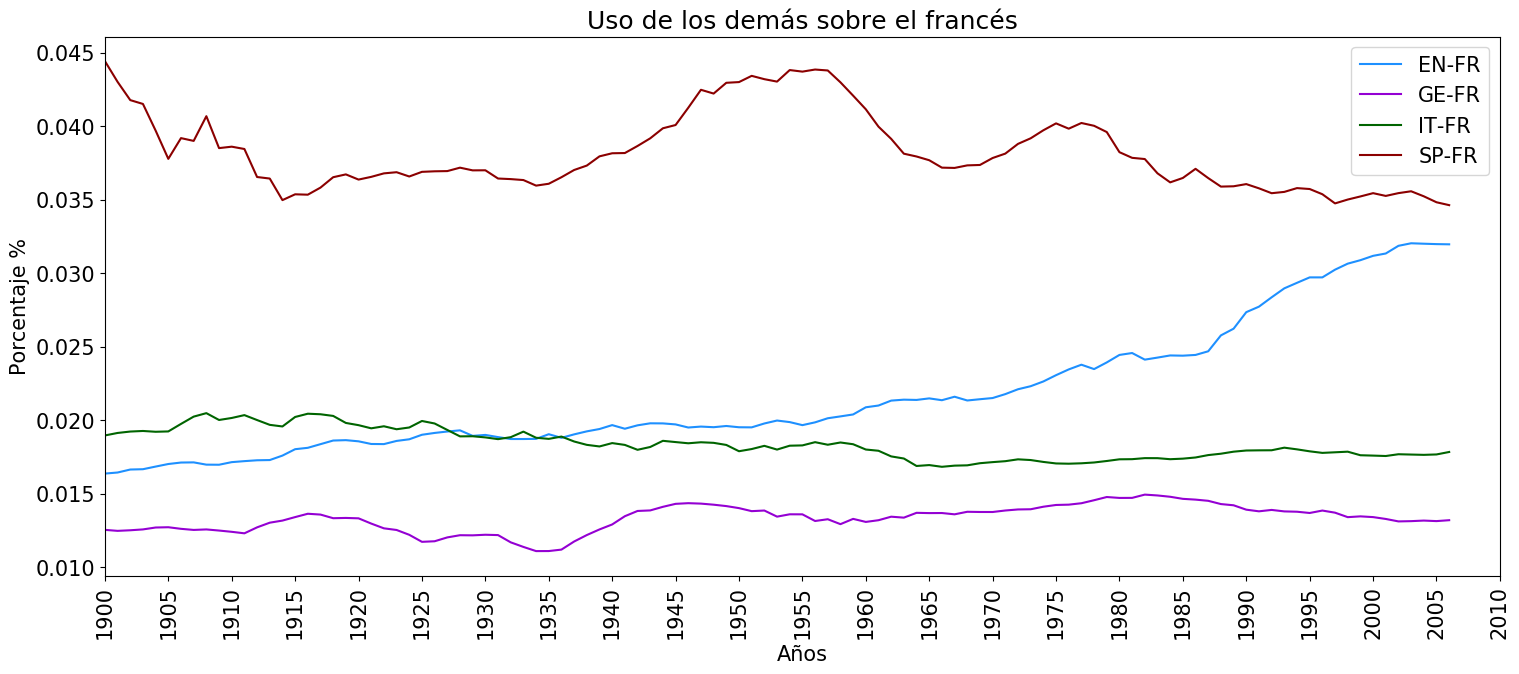
\includegraphics[scale=.38]{Cap_3/PF2_S2_FR.png}
		\caption{}
		\label{fig:ST_FR_b}
	\end{subfigure}
	
\end{figure}

A pesar de que el idioma que más préstamos toma del francés es el inglés,  el idioma que más utiliza el francés ha sido el italiano,  aspecto que se mantuvo durante todo el siglo del análisis.  Recapitulando lo comentado en los análisis de los préstamos,  el peso que tuvo la segunda guerra fue un detonante para que el uso entre los idiomas cambiase durante y posterior al conflicto,  en el caso del alemán y del inglés,  el empleo del francés en ellos aumentó tras finalizar el conflicto.  A pesar de que el español y el francés provienen de la familia de las lenguas romances,  el uso del francés en el español se ha mantenido sin mayores alteraciones.

El caso de cómo son utilizados los demás idiomas en el francés,  hay un dominio de las palabras con origen español, seguido por las de origen inglés; aunque el español ha sido el más empleado en el francés,  el inglés a partir de 1940 comienza a ser más frecuentado,  recortando en cado año la diferencia con el español,  siendo en la última parte del estudio  menor al 0.05$\%$, incluso si la base de datos abarcara más años posteriores al 2009, es probable que el uso el inglés pase al español. 


\newpage
\subsection{Alemán}

\begin{figure}[h!]
	
	\begin{subfigure}{}
		\centering
		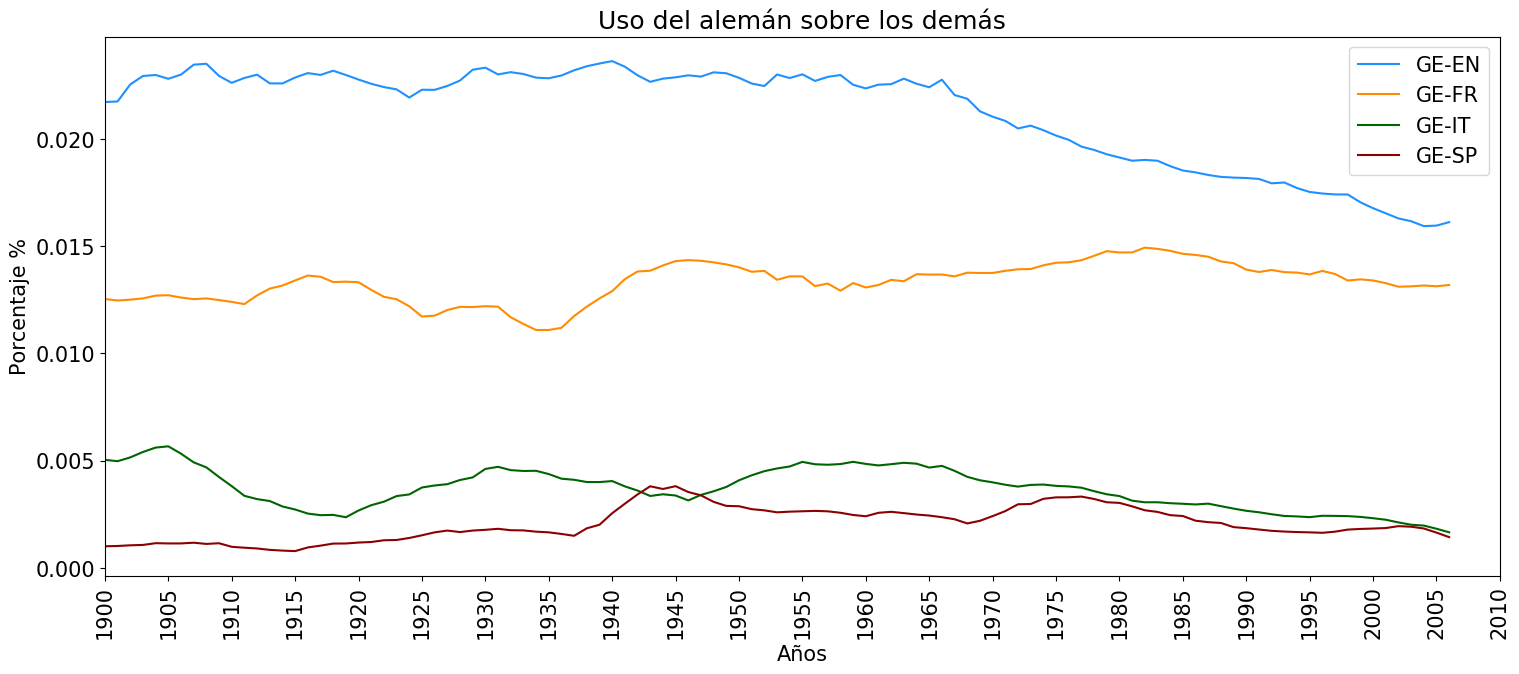
\includegraphics[scale=.38]{Cap_3/PF1_S2_GE.png}
		\caption{}
		\label{fig:ST_GE_a}
	\end{subfigure}
	
	\begin{subfigure}{}
		\centering
		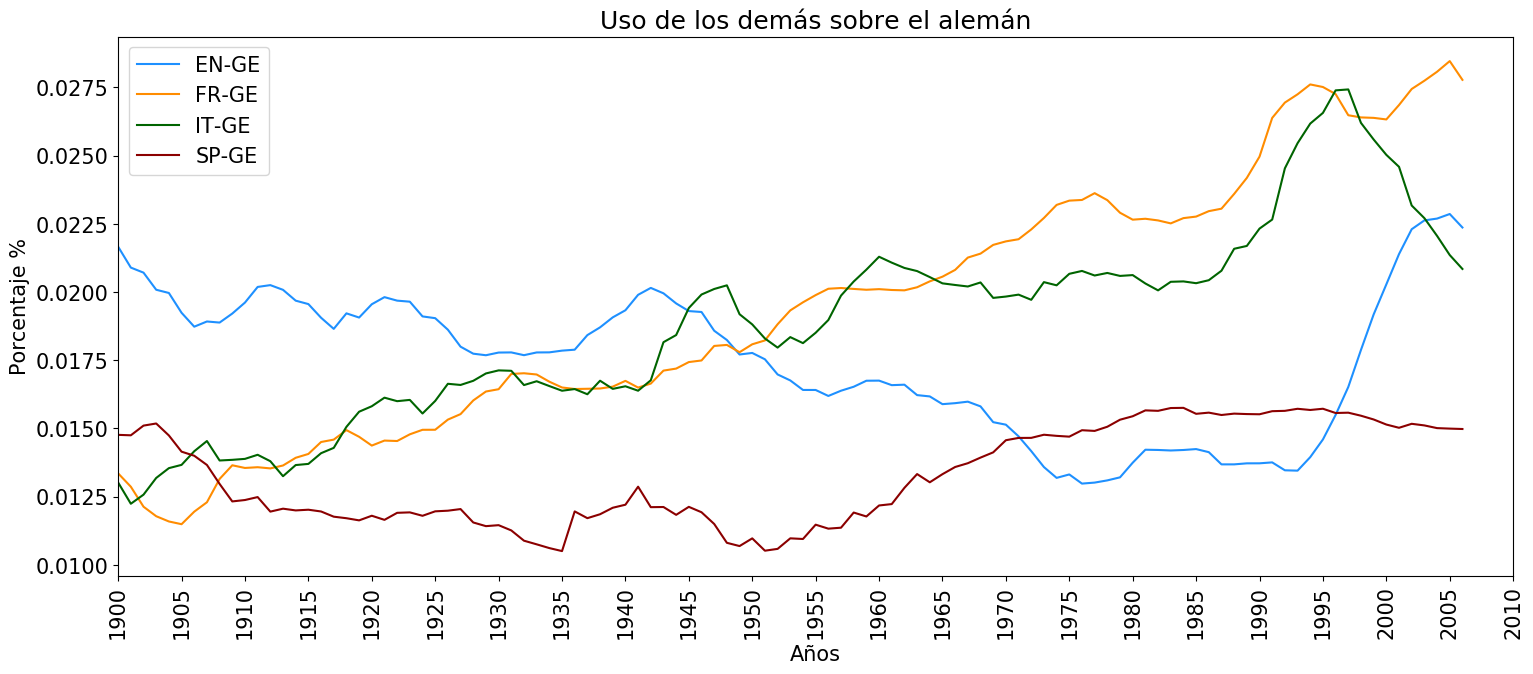
\includegraphics[scale=.38]{Cap_3/PF2_S2_GE.png}
		\caption{}
		\label{fig:ST_GE_b}
	\end{subfigure}
	
\end{figure}

De acuerdo a la tabla [XXX],  el inglés, el francés, el italiano y el español, son en ese orden idiomas que más préstamos tienen provenientes del alemán, a pesar de que el alemán sea en cada uno el idioma del que menos se componen.  El orden de los idiomas que más emplean el alemán es el mismo que los idiomas que más se componen del alemán, siendo el único caso donde la mayor cantidad es también el mayor uso. Una razón de esta característica es que tanto el alemán como el inglés provienen de la misma familia lingüística, la germánica,  siendo más comunes las palabras entre ellos  que con las lenguas romances.

El sentido de cómo se utilizan los demás idiomas en el alemán, no presenta la característica anterior,   donde se ha alternado entre el inglés, el francés y el italiano el idioma que es más utilizado en el alemán.  El inglés fue el más empleado en la primera mitad del siglo, mientras que posterior a la guerra que ha sido el común detonante para que se altere el uso de un idioma en otro,  francés e italiano rolaron el papel del idioma más común en el alemán. 


\newpage
\subsection{Italiano}

\begin{figure}[h!]
	
	\begin{subfigure}{}
		\centering
		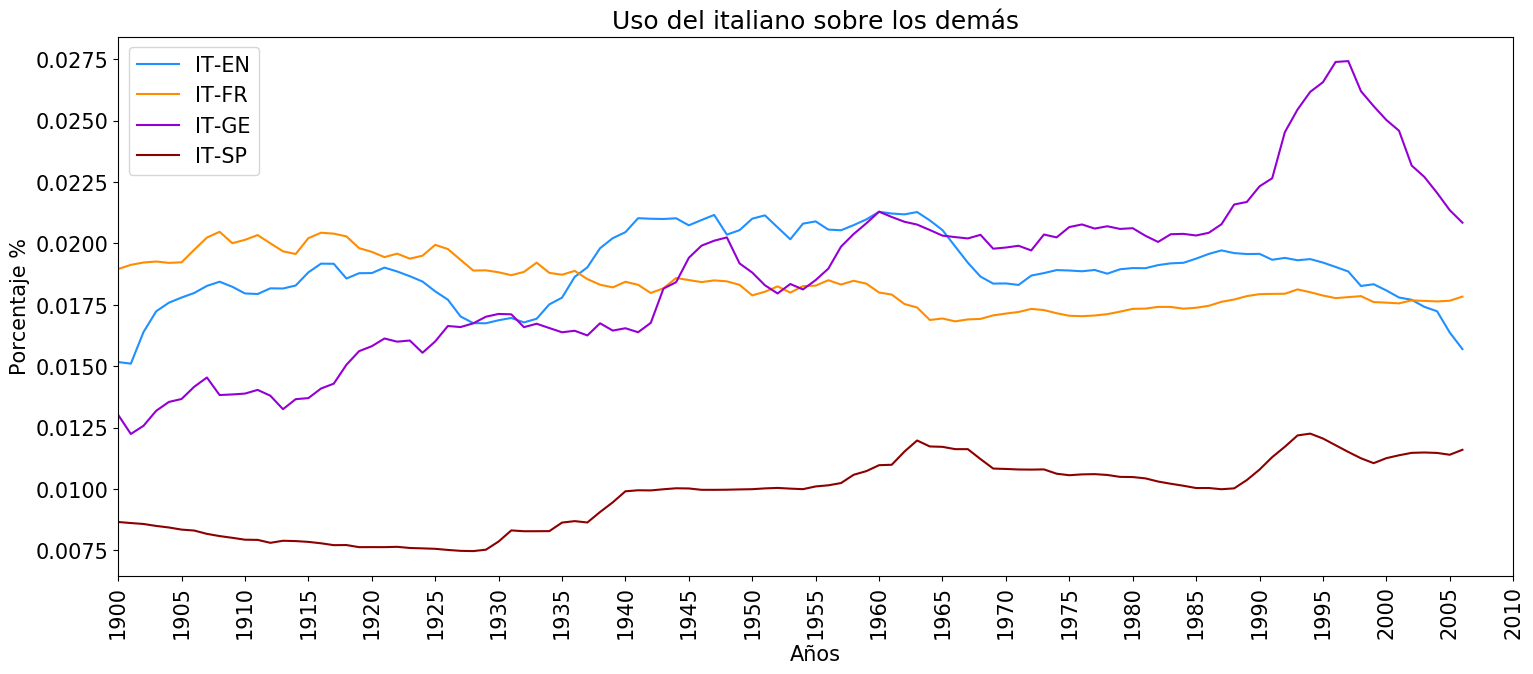
\includegraphics[scale=.38]{Cap_3/PF1_S2_IT.png}
		\caption{}
		\label{fig:ST_IT_a}
	\end{subfigure}
	
	\begin{subfigure}{}
		\centering
		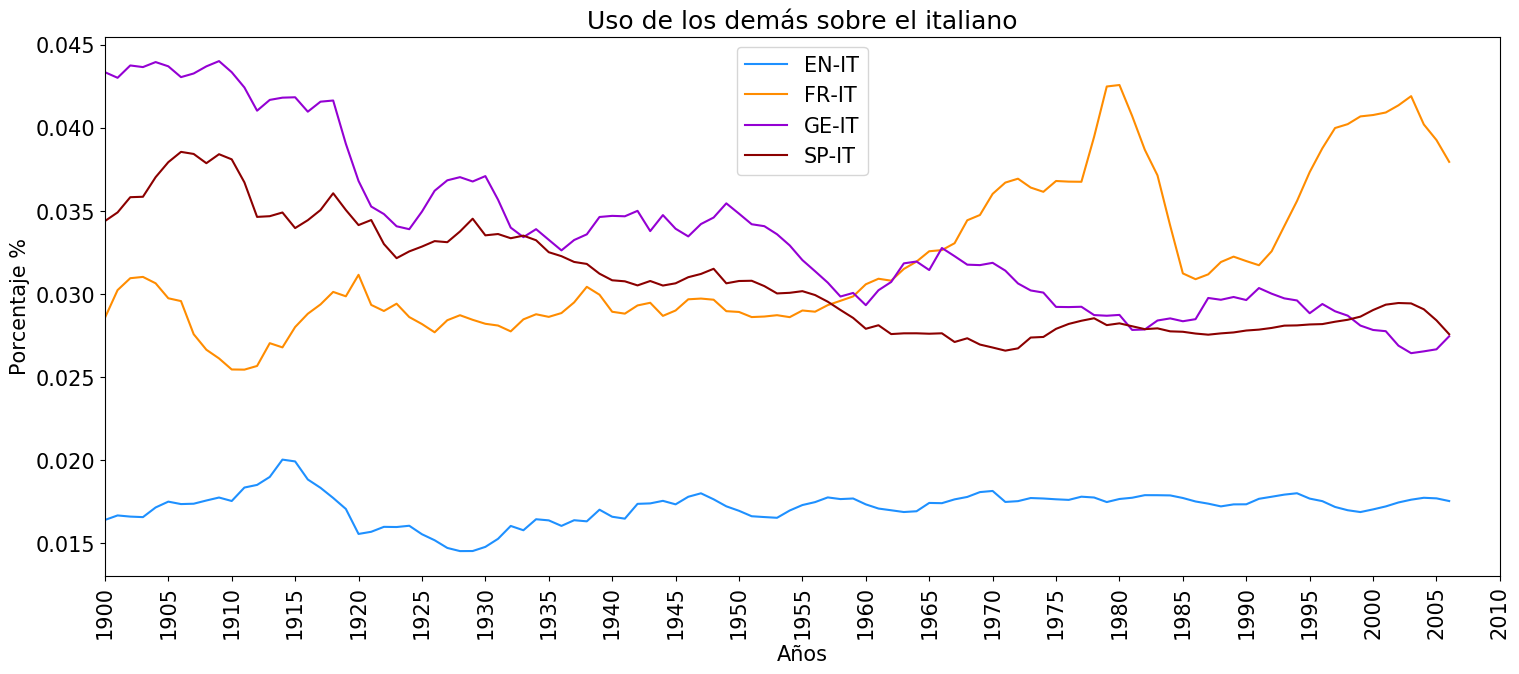
\includegraphics[scale=.38]{Cap_3/PF2_S2_IT.png}
		\caption{}
		\label{fig:ST_IT_b}
	\end{subfigure}
	
\end{figure}

Los idiomas en los que el italiano ha tenido una mayor influencia han sido el inglés, el francés y el alemán pese a que el español es el idioma que más préstamos contiene del  italiano,  circunstancias como la cercanía geográfica entre los países de habla alemán con Italia alude al  mayor uso del italiano en este idioma a partir de  la segunda mitad del siglo,  respecto al inglés,  la intervención de personajes  italianos en la historia y el hecho de que el inglés se compone de palabras de origen grecolatino,  permite que el italiano sea una lengua fuerte en el inglés;  las afirmaciones anteriores se han respaldado en que las palabras de contenido han sido previamente relacionadas  a sucesos donde han intervenido estos países.


La forma de actuar de los demás idiomas en el italiano no es recíproca a la forma en que el italiano interviene en ellos.  El caso del inglés es particular, porque a pesar del impacto que ha manifestado el inglés en los demás idiomas  en los últimos cincuenta años por la globalización,  en el italiano ha sido el único idioma donde no ha sido dominante en algún punto, o donde no ha crecido más que los demás.  El alemán ha sido más importante al comienzo del siglo y decae tras finalizar la segunda guerra mundial, para imponerse el francés como el idioma que más es utilizado en el italiano. 


\newpage
\subsection{Español}


\begin{figure}[h!]
	
	\begin{subfigure}{}
		\centering
		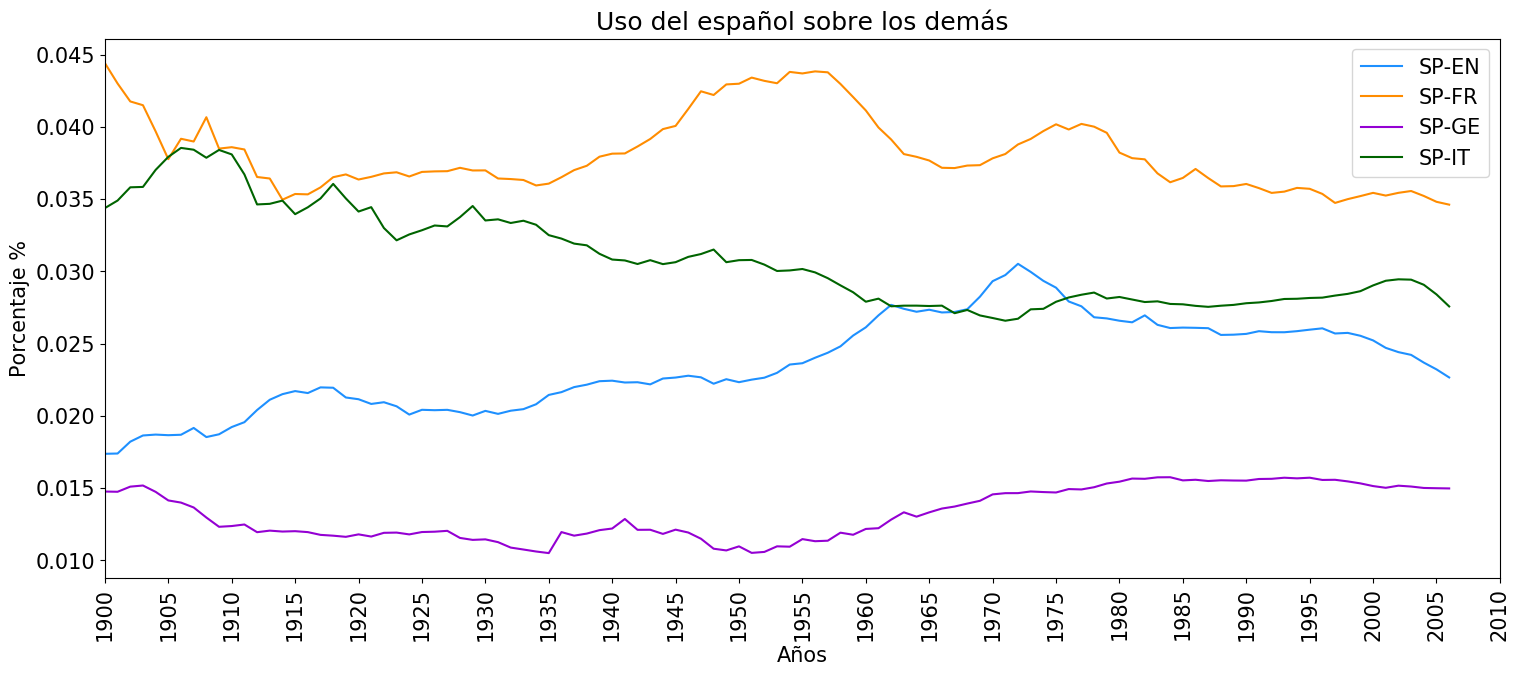
\includegraphics[scale=.38]{Cap_3/PF1_S2_SP.png}
		\caption{}
		\label{fig:ST_SP_a}
	\end{subfigure}
	
	\begin{subfigure}{}
		\centering
		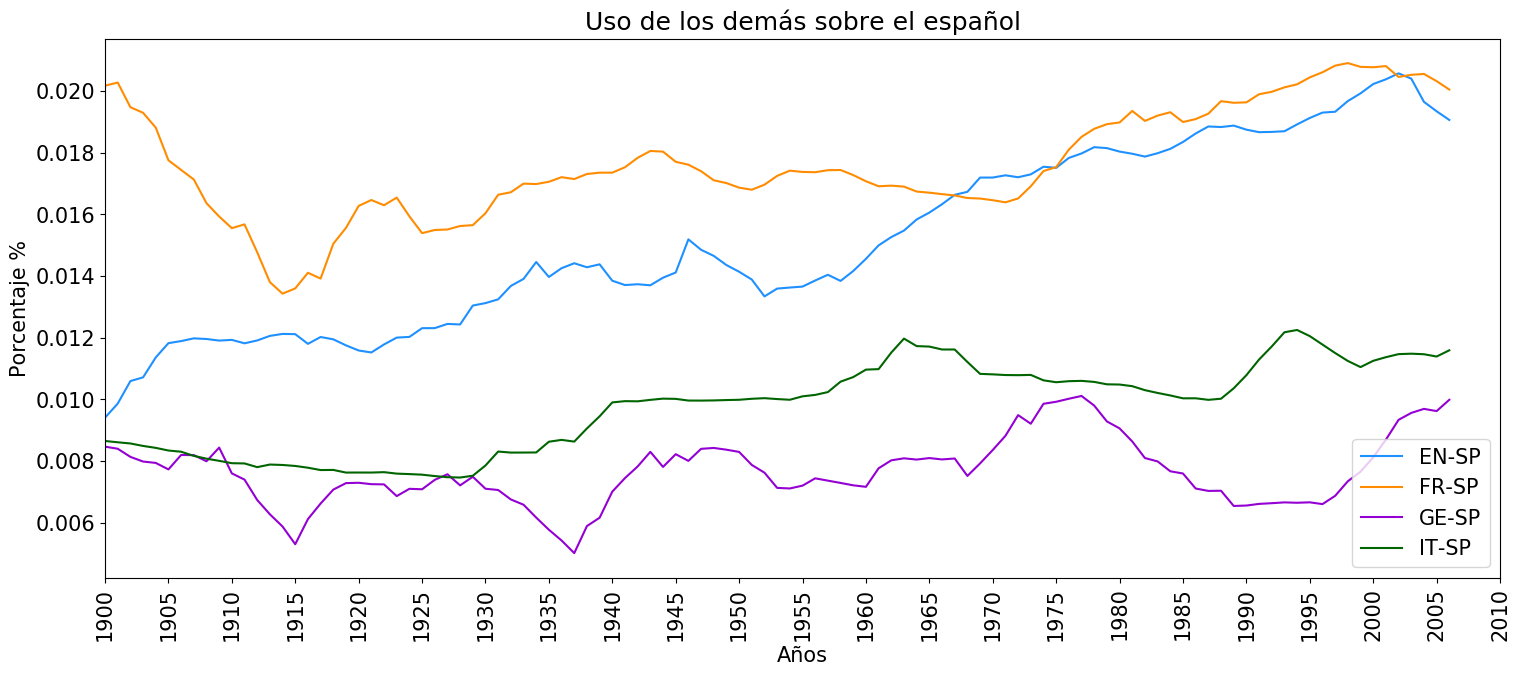
\includegraphics[scale=.38]{Cap_3/PF2_S2_SP.png}
		\caption{}
		\label{fig:ST_SP_b}
	\end{subfigure}
	
\end{figure}


Entre los gráficos de uso entre un determinado idioma y el español, se observó que el español ha sido más influyente en los demás que los demás en él,  siendo el francés el idioma donde el español es más utilizado, a pesar de que la cantidad de préstamos que llegan al italiano es mayor.   Ya se han mencionado factores que condicionan la forma de las gráficas, siendo la más evidente, el provenir de la misma familia lingüística al ser el español más utilizado en el francés y el italiano. 

Entre la forma en la que se usan los préstamos de los demás idiomas en el español,  en los últimos cincuenta años, la mayor influencia se ve compartida entre las palabras que vienen del francés y  del inglés;  la familia de las lenguas romances y sus similitudes hacen posible que el francés tome relevancia, mientras que la globalización y el crecimiento económico de países de habla inglesa hace relevante al inglés en el español.   Por otro lado,  el italiano y el alemán  no presentan el mismo crecimiento que el francés y el inglés,  por parte del italiano se ha comentado que al ser lengua romance al igual que el español,  el periodo donde los préstamos modificaban el uso del idioma receptor pudiese ser tan antiguo como el surgimiento de los idiomas,  por ello comparten gran cantidad de palabras pero estas no alteran el comportamiento del receptor; mientras que en el caso del alemán la poca relación con el español y el no haber existido un evento que los involucren,  hace que estos idiomas no se hayan mezclado como los demás,  por ejemplo alrededor de 1915 y 1935,  el alemán en el español es casi nulo, a pesar de que en esas fechas se desarrollaron las grandes guerras.


\newpage

\section{¿Qué hace posible la Influencia?}

Al tratar de asociar los préstamos (tanto nuevos como acumulados) a hechos que expliquen periodos donde un idioma aporta más palabras y donde el uso entre idiomas se ve alterado, se han encontrado distintos detonantes para que estas características sucedan:

\begin{itemize}
	\item \textbf{Acontecimientos históricos:} Están involucrados países o personajes que hablen determinados idiomas, si el acontecimiento es relevante el intercambio de palabras y las alteraciones en el uso ocurrirán. El hablar de estos hechos abarca temas bélicos, políticos, económicos y de desarrollo científico e industrial. 
	
	\item \textbf{Acontecimientos históricos:} Los países que se encuentren cercanos presentarán intercambios e influencia en el lenguaje y la cultura de sus habitantes.  Este motivo no solo se ve reflejado en el lenguaje escrito en los libros, sino en los diferentes medios de comunicación y relación entre las personas,  sin embargo al tratar unicamente libros se encuentra más información histórica de eventos que fueron prolongados, si se tratasen los periódicos, la información puede ser más espontánea o del día a día de las regiones. 
	
	\item \textbf{Acontecimientos históricos:} Por la similitud de palabras o por provenir de una etimología común, los préstamos entre lenguas de la misma familia son más comunes y adaptables al idioma receptor. El que dos lenguajes de distintas familias tengan modificaciones en el uso de los préstamos se puede deber a un acontecimiento histórico o a la proximidad geográfica. 
	
	
\end{itemize}

Pese a que en su mayoría los factores que originan los intercambio y las alteraciones son algunos de los mencionados anteriormente, también se encontraron casos donde no fue posible asociar las palabras. 

La información  de las causas de la influencia y las relaciones de los préstamos de las dos secciones previas,  han permitido diferenciar tres tipos de influencia: 

\begin{description}
	
	\item[Influencia inmediata:] Sucede en un periodo corto de años y ocurre durante un evento histórico o pocos años después de su finalización.  
	
	\item[Influencia continua:] Caracterizada por un periodo prolongado de tiempo donde ocurren los intercambios y las alteraciones en el uso
	
	\item[Influencia retomada:] Ocurre al suceder un evento que retoma ideas o hechos que ocurrieron en el pasado, siendo nuevamente relevantes los intercambios y alteraciones. 
	
\end{description}


